\documentclass{standalone}

\usepackage{tikz}
\usetikzlibrary{arrows}
\usetikzlibrary{decorations.markings}
\usepackage{standalone}

\begin{document}

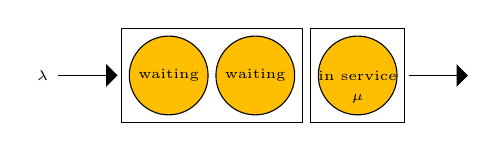
\begin{tikzpicture}

\draw (0, 0) rectangle (2.3, 1.2);
\draw (2.4, 0) rectangle (3.6, 1.2);

\draw[fill=orange!50!yellow] (0.6, 0.6) circle [radius=0.5] node {\tiny waiting};
\draw[fill=orange!50!yellow] (1.7, 0.6) circle [radius=0.5] node {\tiny waiting};
\draw[fill=orange!50!yellow, align=center] (3, 0.6) circle [radius=0.5] node {\tiny in service};

\draw[-triangle 90] (-0.8, 0.6) -- (-0.05, 0.6);
\draw[-triangle 90] (3.65, 0.6) -- (4.4, 0.6);

\node at (-1, 0.6) {\tiny $\lambda$};
\node at (3, 0.3) {\tiny $\mu$};

\end{tikzpicture}

\end{document}
